\documentclass[a4paper,review,12pt]{elsarticle}

\usepackage[utf8]{inputenc}
\usepackage[T5]{fontenc}
\usepackage{amsmath}
\usepackage{amssymb}
\usepackage{booktabs}
\usepackage{tabularx}
\usepackage{array}
\usepackage{graphicx}
\usepackage{xcolor}
\usepackage{float}
\usepackage{microtype}
\usepackage{xurl}
\usepackage[hidelinks]{hyperref}

\definecolor{paceblue}{HTML}{0072B2}
\definecolor{pacesky}{HTML}{56B4E9}
\definecolor{pacegreen}{HTML}{009E73}
\definecolor{paceorange}{HTML}{E69F00}
\definecolor{pacevermillion}{HTML}{D55E00}
\definecolor{pacepurple}{HTML}{CC79A7}

\journal{Image and Vision Computing}

\newcommand{\method}{PACE-Seg}
\newcommand{\miou}{mIoU}
\newcommand{\etal}{et al.}
\setlength{\emergencystretch}{2em}
\hfuzz=3pt

\begin{document}

\begin{frontmatter}

\title{PACE-Seg: Hardware-Cost-Conditioned Elastic Semantic Segmentation with Calibrated Risk Routing for Edge Accelerators}

\author{D\~{u}ng Nguy\~{\^{e}}n}

\begin{abstract}
Edge semantic segmentation faces two coupled uncertainties: visual difficulty changes under adverse conditions, and model cost changes across accelerator architectures. We present \method, a compiler-safe elastic model with four statically deployable capacities and a runtime policy that combines measured route latency with candidate-specific error estimates from one low-cost entropy probe. Experiments use Cityscapes, four ACDC conditions, and four edge devices. The capacities span $110.2\times$ in FLOPs but only $10.3$--$19.5\times$ in measured candidate latency, so a proportional FLOPs proxy fails to reproduce measured budget choices. The largest elastic capacity remains within 1.1 \miou{} points of a similarly sized independently trained Fast-SCNN on every evaluated split. In deployment-matched held-out replay with complete warm-route costs on TensorRT/CUDA and Hailo-8, the budget-constrained policy outperforms or matches rank escalation in 70 of 74 fair operating cells, with a macro gain of 0.0284 \miou{}; it produces no budget-violating cell, compared with 46 of 120 for rank escalation. Pooled calibration gives a similar result. The operating cells are correlated, and the two backends share segmentation predictions.
\end{abstract}

\begin{keyword}
semantic segmentation \sep elastic neural networks \sep dynamic inference \sep uncertainty calibration \sep edge acceleration \sep hardware-aware deployment
\end{keyword}

\end{frontmatter}

\section{Introduction}
\label{sec:introduction}

Edge semantic segmentation faces two coupled uncertainties. Fog, night, rain, and snow alter visual difficulty, while heterogeneous accelerators assign different costs to the same model. Static networks expose one operating point, and elastic networks expose several capacities without deciding which capacity is warranted for an image under a measured deployment budget.

\method{} addresses this joint problem with four static capacities extracted from one compiler-safe elastic model. A tiny prediction supplies an image-level entropy feature, candidate-specific calibrators estimate expected error, and measured complete-route costs define the hardware-feasible set.

The experiments ask whether measured hardware cost is necessary for selection (RQ1), whether shared elastic training preserves segmentation quality (RQ2), and whether candidate-specific risk routing improves the quality--latency trade-off under a measured budget (RQ3). Quantization-aware training remains a secondary deployment study reported in the supplement.

The contributions are as follows:
\begin{enumerate}
    \item A compiler-safe elastic segmentation model exposes four width--depth--resolution capacities as separately compilable static graphs from one shared training process.
    \item A measured-cost candidate set replaces FLOPs with observed deployment latency when constructing hardware-feasible choices.
    \item A candidate-specific calibrated-risk policy maps one inexpensive visual probe to candidate error estimates and selects capacity under an explicit hardware budget.
\end{enumerate}

Figure~\ref{fig:dataset-overview} and Table~\ref{tab:study-setting} summarize the study.

\begin{figure}[H]
\centering
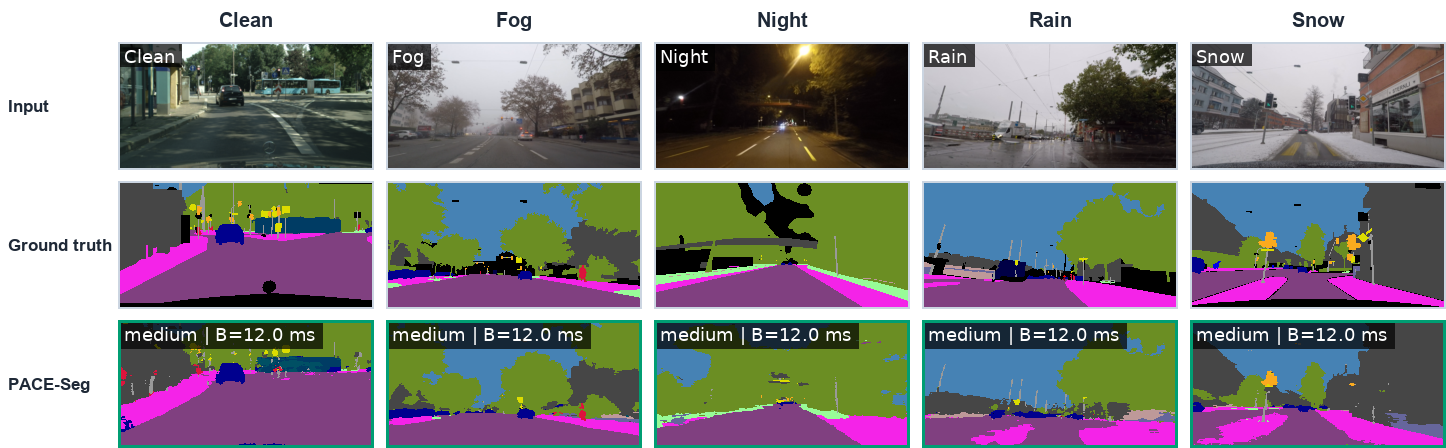
\includegraphics[width=\textwidth]{figures/fig1_data_gt_routed.png}
\caption{Visual domains and routed outputs. Columns show clean Cityscapes and ACDC fog, night, rain, and snow; rows show the input, 19-class ground truth, and configured policy-D output. Each image is the deterministic held-out median-error representative for its split. All five select medium at the displayed E3 operating point, so the panel introduces the task and visual shift rather than comparing routing policies.}
\label{fig:dataset-overview}
\end{figure}

\begin{table}[H]
\centering
\caption{Study setting at a glance. Candidate-only latency is measured on four devices; complete routed latency, including probing and decision overhead, is measured on the two primary accelerator backends.}
\label{tab:study-setting}
\small
\begin{tabularx}{\textwidth}{@{}>{\bfseries}lX@{}}
\toprule
Component & Evaluated setting \\
\midrule
Visual domains & Cityscapes clean and ACDC fog, night, rain, and snow \\
Prediction task & Semantic segmentation over the 19 Cityscapes train classes \\
Elastic choices & Tiny, small, medium, and large static capacities \\
Candidate-cost devices & E1, E2, E3, and E5 \\
Complete-route backends & E1 Hailo-8 and E3 TensorRT/CUDA \\
Router protocol & Alternating fit/held-out validation halves; three training runs \\
\bottomrule
\end{tabularx}
\end{table}

The same label space appears under substantially different visibility and illumination. Hardware feasibility is evaluated separately from visual risk; the reported operating cells are correlated evaluations rather than independent replications.

\section{Related work}
\label{sec:related}

\subsection{Efficient and real-time semantic segmentation}

BiSeNet, STDC, PIDNet, SegFormer, and OffSeg improve the static accuracy--efficiency trade-off through spatial-detail, context, boundary, attention, and offset mechanisms~\cite{yu2018bisenet,fan2021stdc,xu2023pidnet,xie2021segformer,zhang2025offseg}. They still commit an image to one deployed operating point.

\subsection{Elastic, slimmable, and once-for-all networks}

Slimmable networks, US-Net, and Once-for-All share parameters across widths or broader depth--width--resolution spaces~\cite{yu2019slimmable,yu2019usnet,cai2020ofa}. SlimSeg and MESS bring shared widths or exits to segmentation~\cite{xue2022slimseg,kouris2022mess}, but do not combine candidate-specific error estimates with a measured complete-route budget.

\subsection{Hardware-aware deployment}

MnasNet established direct latency as a hardware-aware search objective~\cite{tan2019mnasnet}; FasterSeg, AutoSegEdge, multi-objective edge NAS, RealtimeSeg, and HARD incorporate platform cost into static segmentation design~\cite{chen2020fasterseg,dou2023autosegedge,dou2024multiobjective,li2023realtimeseg,kwon2024hard}. \method{} instead selects among fixed candidates at runtime. RQ1 concerns a proportional FLOPs proxy, not learned latency prediction in general.

\subsection{Uncertainty and adaptive inference under adverse conditions}

Dynamic Routing, Anytime Dense Prediction, and MESS allocate segmentation computation according to the input~\cite{li2020dynamic,liu2022anytime,kouris2022mess}. Segmentation confidence also changes with capacity and domain shift~\cite{wang2023calibrating,dejorge2023reliability}. On Cityscapes and ACDC~\cite{sakaridis2021acdc}, \method{} maps one tiny-probe entropy score to a separate monotonic error estimate for each candidate; these estimates do not provide formal risk control.

\subsection{Positioning of PACE-Seg}

Table~\ref{tab:related-positioning} separates candidate construction, selection time, cost, and risk among the closest directions.

\begin{table}[H]
\centering
\caption{Mechanism-level positioning relative to representative primary work. Entries summarize the stated operating mechanism rather than rank methods or claim exhaustive coverage. ``Complete route'' includes the probe, risk computation, policy decision, backend dispatch or activation, and any additional candidate inference.}
\label{tab:related-positioning}
\scriptsize
\setlength{\tabcolsep}{1.4pt}
\renewcommand{\arraystretch}{1.08}
\begin{tabular}{@{}>{\raggedright\arraybackslash}p{2.3cm}>{\raggedright\arraybackslash}p{2.0cm}>{\raggedright\arraybackslash}p{1.45cm}>{\raggedright\arraybackslash}p{2.1cm}>{\raggedright\arraybackslash}p{2.0cm}>{\raggedright\arraybackslash}p{3.35cm}@{}}
\toprule
Method & Candidates & Selection & Cost & Risk & Budget; deployed form \\
\midrule
Once-for-All~\cite{cai2020ofa} & Elastic subnetworks & Design & Latency predictor & None & Design constraint; static subnet \\
SlimSeg~\cite{xue2022slimseg} & Slimmable widths & Configured & Efficiency setting & None & No hard measured budget; static width \\
MESS~\cite{kouris2022mess} & Multi-exit network & Per image & Exit latency & Exit confidence & No complete-route constraint; multi-exit graph \\
Dynamic Routing~\cite{li2020dynamic} & Multi-scale paths & Per image & Compute penalty & Learned gates & No measured accelerator constraint; dynamic paths \\
AutoSegEdge~\cite{dou2023autosegedge} & Searched architecture & Design & FLOPs + device latency & None & Search constraint; static architecture \\
\method{} & Four elastic capacities & Per image & Measured complete route & Candidate-specific error & Hard measured budget; static compiled engines \\
\bottomrule
\end{tabular}
\end{table}

The gap is per-image selection with candidate-specific error estimates and a budget defined by the measured complete accelerator route. \method{} addresses this intersection with static compiled candidates; its contribution is integrative rather than a claim that its individual components are new.

\section{Method}
\label{sec:method}

\subsection{System overview}
\label{sec:overview}

Shared training produces four capacities that are exported as independently compilable static graphs. At inference, the tiny candidate supplies a segmentation and one entropy feature; candidate-specific calibrators estimate error, measured route costs define feasibility, and the policy selects a feasible capacity. Figures~\ref{fig:candidate-family}--\ref{fig:input-output-pipeline} show the family, inference path, and one complete decision.

\subsection{Compiler-safe elastic candidate family}
\label{sec:elastic}

Tiny, small, medium, and large jointly vary width multiplier (0.25, 0.50, 0.75, 1.00), repeated-block depth (2, 3, 4, 6), and input resolution ($384\times192$, $512\times256$, $768\times384$, $1024\times512$). They share convolutional weights through active-channel slicing and retain level-specific batch-normalization state. Standard operators and fixed-factor resizing permit each level to be exported as a static graph, so routing selects an engine before execution rather than introducing data-dependent control flow inside the graph.

\begin{figure}[H]
\centering
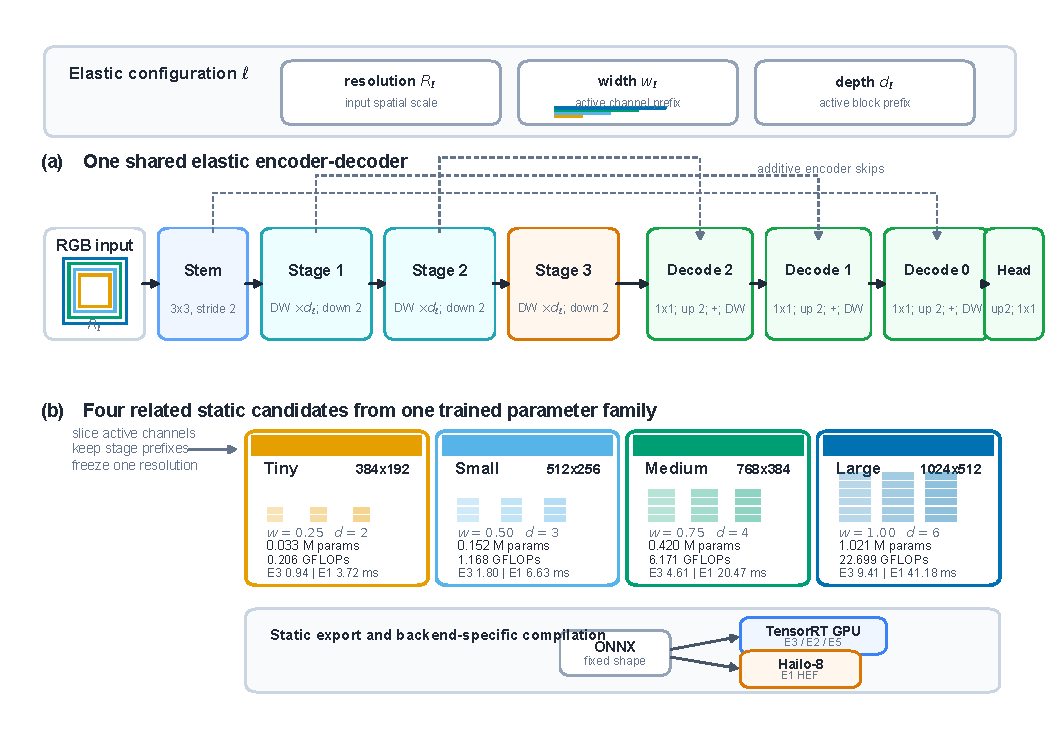
\includegraphics[width=\textwidth]{figures/fig2_candidate_family.pdf}
\caption{Code-audited elastic architecture and static extraction. (a) The active inference path uses a stem, three downsampling depthwise-separable encoder stages, three top-down decoder stages with additive encoder skips, and a 19-class head. Resolution, active-channel prefix, and active-block prefix define elasticity. (b) Tiny through large freeze those axes into four related static graphs, exported through fixed-shape ONNX to TensorRT GPU or Hailo-8. Reported E3/E1 values are candidate-only p95 latency; complete route costs are measured separately.}
\label{fig:candidate-family}
\end{figure}

All four capacities are extracted from one shared model. Their measured latency scaling differs from GFLOPs and between backends.

\subsection{Measured-cost candidate set}
\label{sec:measured-cost}

For hardware $h$, candidate $l$ has measured route cost $t_{h,l}$. Candidate-only measurements characterize hardware scaling; complete-route measurements include the probe, risk and policy computation, dispatch or activation, and any additional inference. The tiny prediction is reused when tiny is selected. Cost enters after training, so a new target requires a measured table rather than segmentation retraining.

\subsection{Candidate-specific visual-risk calibration}
\label{sec:calibration}

Let the tiny candidate produce logits $z(x)$. The raw probe score is mean pixel entropy,
\begin{equation}
s(x)=\frac{1}{|\Omega|}\sum_{u\in\Omega}-\sum_{c=1}^{C}p_{u,c}\log\max(p_{u,c},10^{-12}),
\label{eq:entropy}
\end{equation}
where $p$ is the softmax of $z$ and $C=19$. For each candidate $l$, a monotonic calibrator $g_l$ maps the same score to observed per-image pixel error. Fitting and deployment compute entropy over all output pixels; ground truth supplies only fit-half targets over non-ignore labels. Ten equal-count score bins provide mean errors, followed by a cumulative-maximum pass. Thus
\begin{equation}
\widehat{r}_l(x)=g_l(s(x))
\label{eq:risk}
\end{equation}
is candidate-specific calibration from shared sensing. The primary analysis configures one calibrator set per condition; a pooled variant removes that condition choice.

\subsection{Hardware-cost-conditioned policy}
\label{sec:policy}

For a target device, candidate $l$ has measured route cost $t_l$, risk target $\tau$, and budget $B$. The proposed policy D forms the feasible set
\begin{equation}
\mathcal{S}_B=\{l:t_l\leq B\}.
\label{eq:feasible}
\end{equation}
If a feasible candidate satisfies $\widehat{r}_l(x)\leq\tau$, D selects the cheapest such candidate; otherwise it selects the feasible candidate with minimum predicted error, breaking ties by lower cost. The evaluated budget grid starts at the cheapest measured route. Policy A escalates by latency rank from one calibrated probe score. We also report pooled D, static and entropy references, and a non-deployable ground-truth oracle.

\begin{table}[H]
\centering
\caption{Routing-policy roles and information access. ``Per condition'' means that the deployment domain is configured before inference; pooled D removes that requirement. The oracle uses held-out ground truth and is not deployable.}
\label{tab:policy-summary}
\small
\resizebox{\textwidth}{!}{%
\begin{tabular}{@{}lcccc l@{}}
\toprule
Policy & Candidate risk & Hard budget & Calibrator & Deployable & Purpose \\
\midrule
Static small/large & No & No & None & Yes & Fixed-capacity references \\
Raw entropy & No & No & None & Yes & Uncalibrated adaptive baseline \\
Policy A: rank escalation & No & No & Per condition & Yes & Rank-based comparator \\
Policy D: configured & Yes & Yes & Per condition & Yes & Primary method \\
Policy D: pooled & Yes & Yes & Pooled & Yes & Condition-agnostic check \\
Oracle & GT error & Yes & None & No & Upper bound only \\
\bottomrule
\end{tabular}%
}
\end{table}

\begin{figure}[H]
\centering
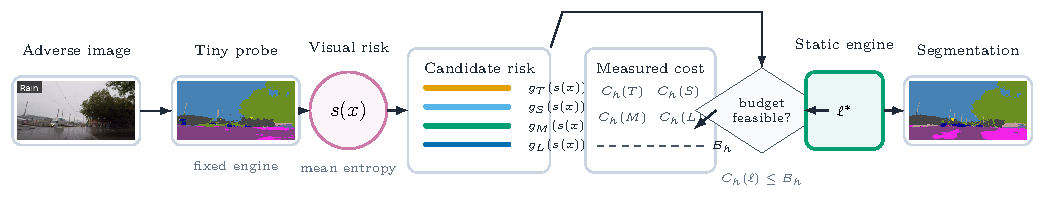
\includegraphics[width=\textwidth]{figures/fig3_condition_probe_routes.pdf}
\caption{Conceptual policy-D inference mechanism. A fixed tiny engine produces the shared entropy score $s(x)$; candidate-specific mappings $g_l$ estimate four risks, while measured costs $C_h(l)$ and budget $B_h$ define feasibility before one static engine is selected. Symbols are schematic; Fig.~\ref{fig:input-output-pipeline} gives one audited numerical instance.}
\label{fig:condition-probe-routes}
\end{figure}

Risk estimation and hardware feasibility remain separate until the final decision. Figure~\ref{fig:input-output-pipeline} instantiates the sequence with audited values.

\begin{figure}[H]
\centering
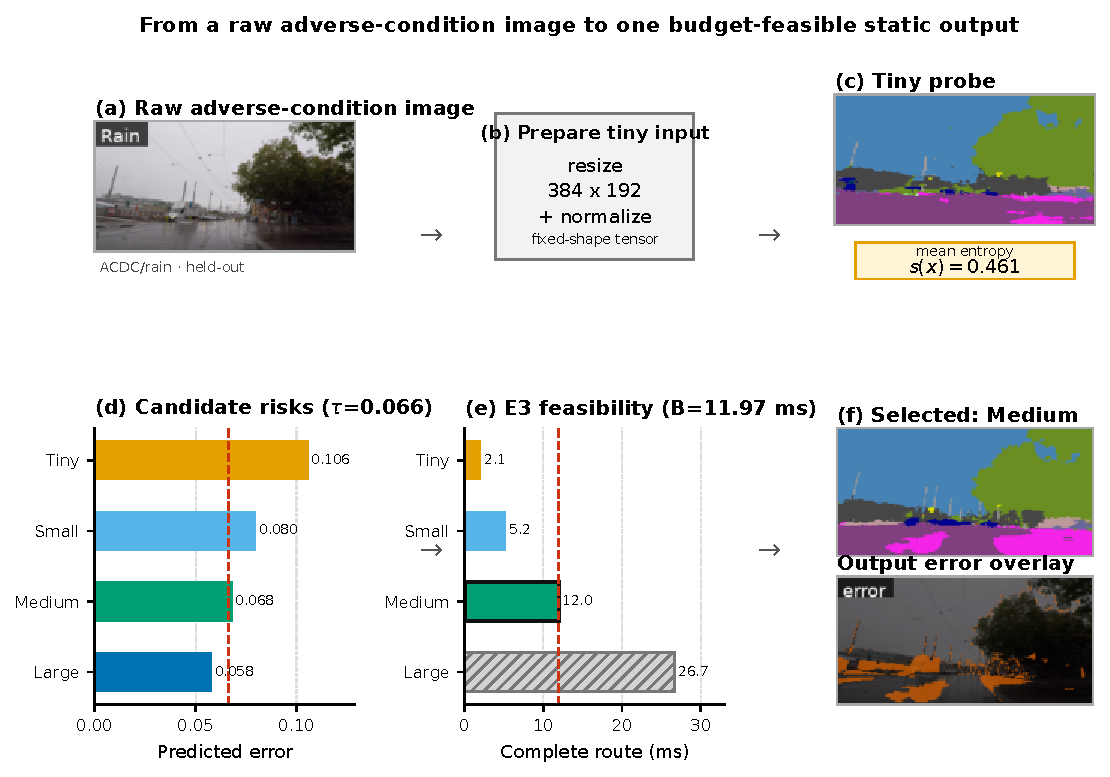
\includegraphics[width=\textwidth]{figures/fig4_input_output_pipeline.pdf}
\caption{One complete policy-D decision on an audited rain image. Tiny-probe entropy maps to candidate-specific expected errors, while measured E3 complete route costs are compared with $B=11.97$~ms. Large is infeasible and no feasible candidate meets $\tau=0.066$, so the minimum-risk feasible fallback selects medium. The final panel overlays output--ground-truth disagreement in orange; this case illustrates the policy and is not an additional evaluation trial.}
\label{fig:input-output-pipeline}
\end{figure}

Risk orders candidates by expected error; measured cost removes unavailable actions.

\subsection{Training}

Elastic training uses the sandwich rule: each step evaluates the smallest and largest levels and one random intermediate level. The largest level receives supervised segmentation loss; smaller levels receive supervised and in-place distillation terms, and a boundary auxiliary term emphasizes semantic transitions. Training runs for 100,000 steps with AdamW, cosine decay, and mixed Cityscapes/ACDC augmentation. Full hyperparameters and the secondary fake-quant protocol are provided in the supplement.

\section{Experimental protocol}
\label{sec:protocol}

\subsection{Datasets and splits}

Cityscapes supplies 2,975 training and 500 validation images~\cite{cordts2016cityscapes}. ACDC supplies 1,600 training and 406 validation images distributed across fog, night, rain, and snow~\cite{sakaridis2021acdc}. Both use the 19 Cityscapes train classes. Each validation split is partitioned by alternating index: even-index images form the calibration and operating-point fit half, and odd-index images form the held-out evaluation half. The study does not use an external test server.

\begin{table}[H]
\centering
\caption{Dataset composition and alternating-index router split. Fit and held-out counts partition each validation subset exactly.}
\label{tab:dataset-splits}
\small
\begin{tabular}{@{}lrrrr@{}}
\toprule
Dataset/condition & Train & Validation & Fit & Held-out \\
\midrule
Cityscapes clean & 2,975 & 500 & 250 & 250 \\
ACDC fog   & 400 & 100 & 50 & 50 \\
ACDC night & 400 & 106 & 53 & 53 \\
ACDC rain  & 400 & 100 & 50 & 50 \\
ACDC snow  & 400 & 100 & 50 & 50 \\
\bottomrule
\end{tabular}
\end{table}

\subsection{Training runs and baselines}

The near-parity comparison uses three supernet runs and three independently trained Fast-SCNN runs. Router results use three separately trained runs (A--C); detailed checkpoint provenance is provided in the supplement and evidence manifest. Fast-SCNN is the matched-capacity RQ2 comparator, while routing references include static candidates, raw entropy, rank-based policy A, configured and pooled policy D, and an oracle.

\subsection{Hardware targets and latency protocol}

Candidate-only latency is measured at batch size one on E1 (Raspberry Pi 5 with Hailo-8), E2 (Jetson Xavier NX), E3 (Jetson AGX Xavier), and E5 (Jetson Orin Nano); NVIDIA devices use TensorRT FP16. Complete warm-route costs are measured on E1 and E3 and include probe inference, risk and policy computation, activation or dispatch, and any additional inference. The analysis combines these measurements with cached trained-model predictions in an offline per-image replay, not an integrated on-device accuracy run. Runtime versions and detailed timing procedures are provided in the supplement.

\subsection{Metrics, seed policy, and unit of analysis}

Segmentation quality is dataset-level \miou{}. Calibration targets per-image pixel error, while routed \miou{} is recomputed from accumulated selected-candidate confusion matrices. An operating cell is defined by run, backend cost table, split, and budget; cells reuse images and predictions and are therefore correlated. Fair A-versus-D cells require A to have no held-out budget violation, and fair-cell quality counts are reported with full-grid violation counts.

\subsection{Fit/held-out separation and leakage safeguards}
\label{sec:split}

Every candidate prediction is cached once per image. Calibrators, risk targets, and operating points use only fit-half scores and errors; held-out labels are read afterward to reconstruct routed \miou{} and budget violations. The same all-pixel entropy feature is used at fitting and deployment. The pooled variant combines only fit halves across conditions, and the oracle uses held-out ground truth only as a non-deployable upper bound. Full threshold selection and leakage audits are documented in the supplement.

\section{Results}
\label{sec:results}

\subsection{RQ1: Why measured hardware cost is necessary}

The four levels require 0.2060, 1.1678, 6.1712, and 22.6992 GFLOPs. Their large-to-tiny ratio is 110.2, whereas measured candidate latency grows by only $10.3$--$19.5\times$ across the four accelerators (Fig.~\ref{fig:flops-latency}). A 10~ms budget selects small on E1/E2, large on E3, and medium on E5. Thus a proportional FLOPs proxy does not recover hardware feasibility in this candidate set.

\begin{figure}[H]
\centering
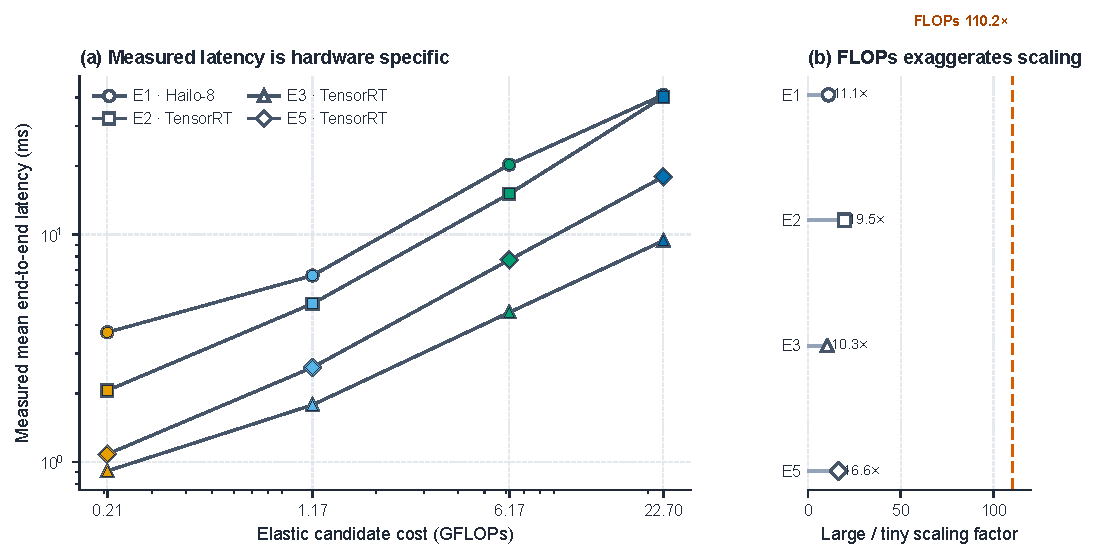
\includegraphics[width=\textwidth]{figures/fig5_flops_vs_latency.pdf}
\caption{Why FLOPs is insufficient as a deployment-cost proxy. Marker shape identifies hardware and color identifies capacity. The $110.2\times$ large-to-tiny compute increase becomes only $10.3$--$19.5\times$ measured latency, so FLOPs preserves order here but not the hardware-specific scale needed to enforce a latency budget.}
\label{fig:flops-latency}
\end{figure}

Across 640 proxy evaluations, same-device proportional fits mis-select 37.5--65\% of budgets, and the worst cross-device transfers reach 85--95\% mis-selection or violation. This result does not address learned latency predictors.

\subsection{RQ2: Whether shared elastic training preserves quality}

Across the three runs per model, the large elastic level differs from independently trained Fast-SCNN by +1.10, +0.21, $-0.65$, $-0.23$, and +0.07 \miou{} points on Cityscapes, fog, night, rain, and snow (Fig.~\ref{fig:rq2}). All means remain inside the prespecified $\pm1.5$-point practical near-parity band, supporting near parity rather than superiority.

\begin{figure}[H]
\centering
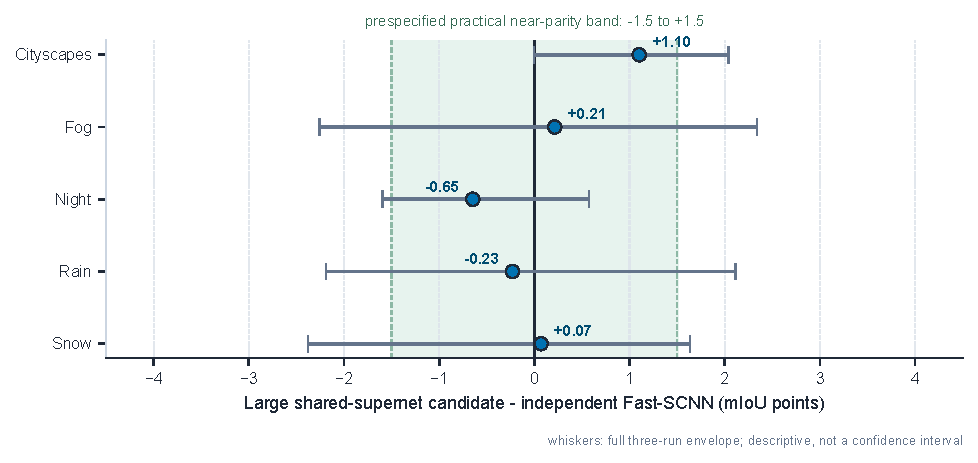
\includegraphics[width=\textwidth]{figures/fig6_rq2_near_parity.pdf}
\caption{Three-run matched-capacity comparison. Points show mean \miou{} differences between the large elastic candidate and independently trained Fast-SCNN; whiskers are the full observed cross-run envelopes, not confidence intervals or paired-seed estimates. All means lie within the prespecified $\pm1.5$-point practical near-parity band, supporting near parity rather than superiority or statistical equivalence.}
\label{fig:rq2}
\end{figure}

\subsection{RQ3: Candidate-specific routing under measured budgets}

RQ3 compares candidate-specific hard-budget policy D with single-score rank policy A using corrected deployment-matched calibration and complete route costs.

\subsubsection{Measured route costs}

Table~\ref{tab:routes} reports the warm-route medians used in replay; each value includes the probe, risk and policy computation, activation or dispatch, and any additional inference.

\begin{table}[H]
\centering
\caption{Median warm end-to-end route cost used in the overhead-aware replay.}
\label{tab:routes}
\begin{tabular}{@{}lrr@{}}
\toprule
Route & E3 TensorRT/CUDA & E1 Hailo-8 \\
\midrule
tiny $\rightarrow$ tiny & 2.07 ms & 34.95 ms \\
tiny $\rightarrow$ small & 5.23 ms & 46.13 ms \\
tiny $\rightarrow$ medium & 11.97 ms & 63.36 ms \\
tiny $\rightarrow$ large & 26.70 ms & 92.68 ms \\
\bottomrule
\end{tabular}
\end{table}

Complete routes range from 2.07 to 26.70~ms on E3 and from 34.95 to 92.68~ms on E1. Candidate-only lookup tables therefore omit substantial backend-specific overhead. The supplement reports the production-path consistency and timing details.

Figure~\ref{fig:routing-decision-example} applies the same audited risk vector and illustrative 60~ms budget to both measured backends.

\begin{figure}[H]
\centering
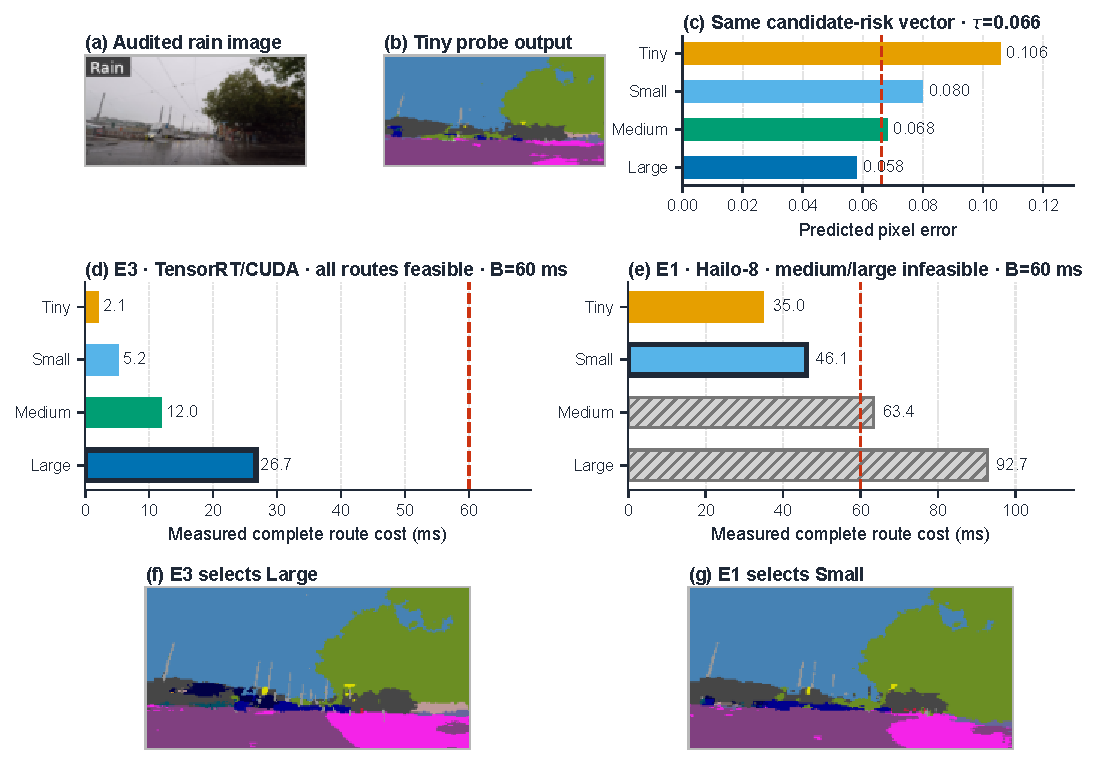
\includegraphics[width=\textwidth]{figures/fig7_routing_decision_example.pdf}
\caption{Same image and risk vector, different measured hardware costs. Under the illustrative 60~ms budget, all E3 routes are feasible and policy D selects large; E1 excludes medium and large and selects small. Only the cost table changes, and the example is a policy illustration rather than an additional evaluation cell.}
\label{fig:routing-decision-example}
\end{figure}

All E3 routes fit the illustrative budget, whereas only tiny and small fit on E1. The changed action is caused by measured hardware cost, not the image or risk estimate.

\subsubsection{Deployment-matched routing result}

The replay recomputes A and D with measured warm-route costs and fit-selected risk targets. One risk grid per run is shared across E1 and E3; configured D uses condition-specific calibrators, while pooled D fits one set from all five fit halves.

\begin{table}[H]
\centering
\caption{Deployment-matched A-versus-D comparison with measured complete route costs. W/T/L uses fair cells; violations use the full grid. Pooled D uses one calibrator set across conditions.}
\label{tab:routerfinal}
\footnotesize
\setlength{\tabcolsep}{3.5pt}
\begin{tabular}{@{}llrrrrrr@{}}
\toprule
Policy & Backend & Fair & W/T/L & Win/tie & Mean $\Delta$ & Policy viol. & A viol. \\
\midrule
Configured D & E3 & 38/60 & 29/7/2 & 94.7\% & +0.0287 & 0/60 & 22/60 \\
Configured D & E1 & 36/60 & 27/7/2 & 94.4\% & +0.0279 & 0/60 & 24/60 \\
Configured D & Overall & 74/120 & 56/14/4 & 94.6\% & +0.0284 & 0/120 & 46/120 \\
Pooled D & Overall & 74/120 & 58/14/2 & 97.3\% & +0.0296 & 0/120 & 46/120 \\
\bottomrule
\end{tabular}
\end{table}

\begin{figure}[H]
\centering
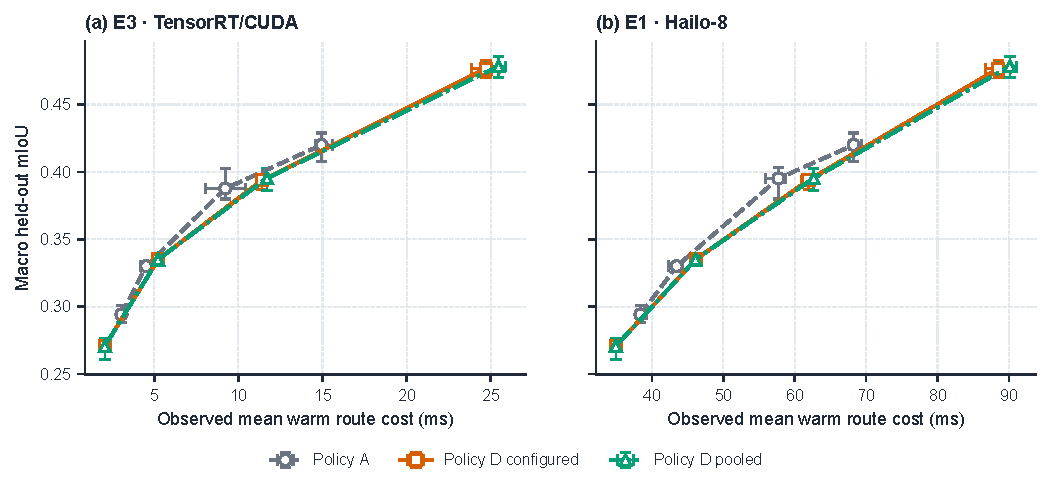
\includegraphics[width=\textwidth]{figures/fig8_router_deployment_matched.pdf}
\caption{Quality versus measured complete warm-route cost after deployment-matched calibration. Points macro-average five held-out splits within each run and then Runs A--C; whiskers show the run-level range, not confidence intervals. Operating cells are correlated and E1/E3 share predictions. Configured and pooled policy D reach higher-quality operating points than rank policy A on both measured backends.}
\label{fig:router-frontier}
\end{figure}

Configured D outperforms or matches A in 70 of 74 fair cells (56/14/4 wins/ties/losses), with a macro +0.0284 \miou{} gap; D has no violating cell across the full 120-cell grid, compared with 46 for A. Pooled D records 58/14/2 and +0.0296 on the same fair subset. The cells are correlated, D enforces feasibility by construction, and E1/E3 share segmentation predictions.

\subsection{Adverse-condition behavior}

The large elastic level averages 0.5311 \miou{} on held-out Cityscapes but 0.3559 on ACDC/night. Probe-signal AURC is also worst at night (three-run mean 0.2416), indicating weaker prediction quality and uncertainty ordering. Figure~\ref{fig:qualitative} shows the five deterministic median-error examples; at the displayed E3 budget, configured D selects medium for all five.

\begin{figure}[H]
\centering
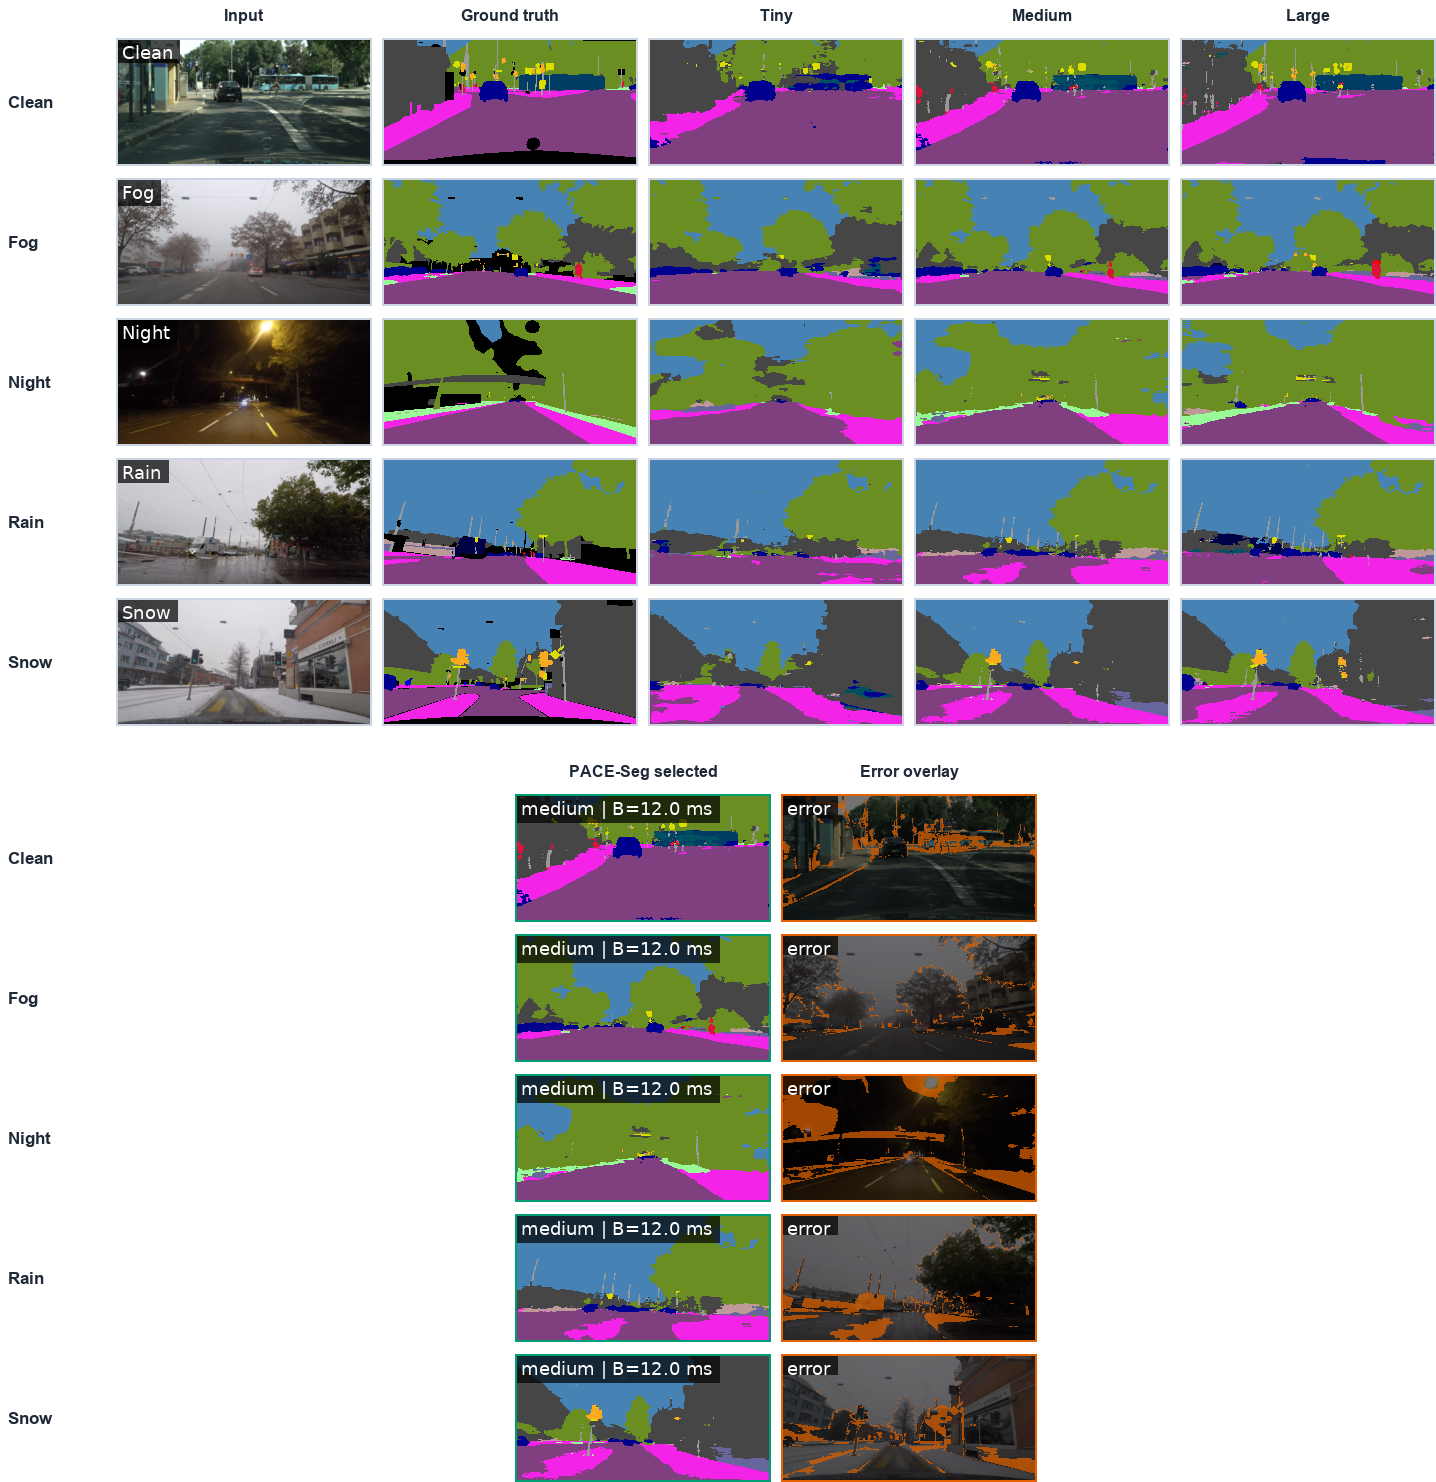
\includegraphics[width=\textwidth]{figures/fig9_qualitative_grid.png}
\caption{Qualitative capacity comparison on the five held-out examples from Fig.~\ref{fig:dataset-overview}. The upper block compares input, ground truth, tiny, medium, and large predictions; the lower block enlarges the configured policy-D output and its error overlay, where orange marks disagreement with ground truth. At $B=11.97$~ms on E3, D selects medium for all five images. Image selection was fixed by median large-candidate pixel error before visual inspection.}
\label{fig:qualitative}
\end{figure}

The four configured-D losses reduce to two Run C operating points replayed on both cost tables; shared predictions prevent interpreting them as independent failures. All four static graphs compile on the primary TensorRT and Hailo-8 paths. Secondary fake-quant results are reported in the supplement and do not establish compiled INT8 accuracy.

\section{Discussion}
\label{sec:discussion}

The experiments separate candidate construction, hardware feasibility, and image-dependent selection. Shared training supplies four static candidates with matched-capacity quality near independently trained Fast-SCNN, while direct measurement determines which candidates fit a deployment budget.

FLOPs fails primarily as a cost scale: the 110.2-fold compute range contracts to a 10.3--19.5-fold latency range. Candidate order may transfer across devices while absolute feasibility changes, so measured cost remains necessary even when some decisions coincide.

Candidate-specific calibration lets one probe score imply different expected errors for different capacities. The results support this design, but calibration cannot recover visual information absent from the probe; night has the weakest uncertainty ordering. Pooled calibration closely tracks configured calibration, although unseen-condition generalization remains untested.

Complete-route measurement changes the deployment conclusion because isolated inference omits uncertainty computation and backend-specific dispatch or activation. Runtime selection should therefore measure the complete path rather than only candidate execution.

\section{Limitations and threats to validity}
\label{sec:limitations}

Calibration is evaluated only on Cityscapes and four ACDC conditions; even pooled calibration uses fit samples from every evaluated condition, so unseen-condition generalization is untested. The alternating validation halves are not an external test set, and repeated budgets reuse images and predictions; the 120 correlated cells are not a statistical sample size.

E1 and E3 use different measured cost tables but share segmentation predictions. Accuracy is replayed offline from trained-model caches, while timing uses compiled graphs with the correct architecture; this is not bit-exact integrated on-device accuracy. D's zero violations are partly structural, and identical latency rankings can yield identical decisions across devices.

The study has four candidates, two complete-route backends, no external energy measurement, and no compiled INT8 accuracy. Fake-quant QAT, cold-start behavior, temporal routing, and systematic class-level error analysis remain secondary or future work.

\section{Conclusion}
\label{sec:conclusion}

\method{} studies elastic semantic segmentation when both visual difficulty and accelerator cost vary. Measured latency is necessary to define feasible candidates, shared training preserves matched-capacity quality, and candidate-specific hard-budget routing improves the descriptive quality--cost trade-off over rank escalation on two accelerators. Pooled calibration retains the result, while correlated cells, shared predictions, offline replay, and the absence of an external test set bound the claim.

\section*{Data and code availability}

The repository records the implementation, experiment reports, canonical result artifacts, and a separate supplement containing detailed provenance, runtime versions, QAT evidence, and extended qualitative and routing analyses. Dataset access remains subject to the Cityscapes and ACDC licenses.

\begin{thebibliography}{99}

\bibitem{yu2018bisenet}
C. Yu, J. Wang, C. Peng, C. Gao, G. Yu, N. Sang,
BiSeNet: Bilateral segmentation network for real-time semantic segmentation,
in: European Conference on Computer Vision, 2018, pp. 325--341.
\url{https://openaccess.thecvf.com/content_ECCV_2018/html/Changqian_Yu_BiSeNet_Bilateral_Segmentation_ECCV_2018_paper.html}.

\bibitem{fan2021stdc}
M. Fan, S. Lai, J. Huang, X. Wei, Z. Chai, J. Luo, X. Wei,
Rethinking BiSeNet for real-time semantic segmentation,
in: IEEE/CVF Conference on Computer Vision and Pattern Recognition, 2021, pp. 9716--9725.
\url{https://openaccess.thecvf.com/content/CVPR2021/html/Fan_Rethinking_BiSeNet_for_Real-Time_Semantic_Segmentation_CVPR_2021_paper.html}.

\bibitem{xu2023pidnet}
J. Xu, Z. Xiong, S.P. Bhattacharyya,
PIDNet: A real-time semantic segmentation network inspired by PID controllers,
in: IEEE/CVF Conference on Computer Vision and Pattern Recognition, 2023, pp. 19529--19539.
\url{https://openaccess.thecvf.com/content/CVPR2023/html/Xu_PIDNet_A_Real-Time_Semantic_Segmentation_Network_Inspired_by_PID_Controllers_CVPR_2023_paper.html}.

\bibitem{xie2021segformer}
E. Xie, W. Wang, Z. Yu, A. Anandkumar, J.M. Alvarez, P. Luo,
SegFormer: Simple and efficient design for semantic segmentation with transformers,
Advances in Neural Information Processing Systems 34 (2021) 12077--12090.

\bibitem{zhang2025offseg}
S.-C. Zhang, Y. Li, Y.-H. Wu, Q. Hou, M.-M. Cheng,
Revisiting efficient semantic segmentation: Learning offsets for better spatial and class feature alignment,
in: IEEE/CVF International Conference on Computer Vision, 2025, pp. 22361--22371.
\url{https://openaccess.thecvf.com/content/ICCV2025/html/Zhang_Revisiting_Efficient_Semantic_Segmentation_Learning_Offsets_for_Better_Spatial_and_ICCV_2025_paper.html}.

\bibitem{yu2019slimmable}
J. Yu, L. Yang, N. Xu, J. Yang, T. Huang,
Slimmable neural networks,
in: ICLR Workshop, 2019.
\url{https://arxiv.org/abs/1812.08928}.

\bibitem{yu2019usnet}
J. Yu, T. Huang,
Universally slimmable networks and improved training techniques,
in: IEEE/CVF International Conference on Computer Vision, 2019, pp. 1803--1811.
\url{https://doi.org/10.1109/ICCV.2019.00189}.

\bibitem{cai2020ofa}
H. Cai, C. Gan, T. Wang, Z. Zhang, S. Han,
Once-for-All: Train one network and specialize it for efficient deployment,
in: International Conference on Learning Representations, 2020.
\url{https://openreview.net/forum?id=HylxE1HKwS}.

\bibitem{xue2022slimseg}
D. Xue, F. Yang, P. Wang, L. Herranz, J. Sun, Y. Zhu, Y. Zhang,
SlimSeg: Slimmable semantic segmentation with boundary supervision,
in: Proceedings of the 30th ACM International Conference on Multimedia, 2022, pp. 6539--6548.
\url{https://doi.org/10.1145/3503161.3548191}.

\bibitem{kouris2022mess}
A. Kouris, S.I. Venieris, S. Laskaridis, N.D. Lane,
Multi-exit semantic segmentation networks,
in: European Conference on Computer Vision, 2022, pp. 330--349.

\bibitem{li2020dynamic}
Y. Li, L. Song, Y. Chen, Z. Li, X. Zhang, X. Wang, J. Sun,
Learning dynamic routing for semantic segmentation,
in: IEEE/CVF Conference on Computer Vision and Pattern Recognition, 2020, pp. 8553--8562.

\bibitem{liu2022anytime}
Z. Liu, Z. Xu, H.-J. Wang, T. Darrell, E. Shelhamer,
Anytime dense prediction with confidence adaptivity,
in: International Conference on Learning Representations, 2022.
\url{https://openreview.net/forum?id=kNKFOXleuC}.

\bibitem{tan2019mnasnet}
M. Tan, B. Chen, R. Pang, V. Vasudevan, M. Sandler, A. Howard, Q.V. Le,
MnasNet: Platform-aware neural architecture search for mobile,
in: IEEE/CVF Conference on Computer Vision and Pattern Recognition, 2019, pp. 2820--2828.

\bibitem{chen2020fasterseg}
W. Chen, X. Gong, X. Liu, Q. Zhang, Y. Li, Z. Wang,
FasterSeg: Searching for faster real-time semantic segmentation,
in: International Conference on Learning Representations, 2020.
\url{https://openreview.net/forum?id=BJgqQ6NYvB}.

\bibitem{dou2023autosegedge}
Z. Dou, D.-Y. Ye, B. Wang, X. Wang, S. Sun,
AutoSegEdge: Searching for the edge device real-time semantic segmentation based on multi-task learning,
Image and Vision Computing 136 (2023) 104719.
\url{https://doi.org/10.1016/j.imavis.2023.104719}.

\bibitem{dou2024multiobjective}
Z. Dou, D.-Y. Ye, B. Wang, X. Wang, S. Sun,
Multi-objective neural architecture search for efficient and fast semantic segmentation on edge,
IEEE Transactions on Intelligent Vehicles 9 (1) (2024) 1346--1357.
\url{https://doi.org/10.1109/TIV.2023.3332594}.

\bibitem{li2023realtimeseg}
Y. Li, C. Yang, P. Zhao, G. Yuan, W. Niu, J. Guan, H. Tang, M. Qin, Q. Jin, B. Ren, X. Lin, Y. Wang,
Towards real-time segmentation on the edge,
Proceedings of the AAAI Conference on Artificial Intelligence 37 (2) (2023) 1339--1347.
\url{https://doi.org/10.1609/aaai.v37i2.25232}.

\bibitem{kwon2024hard}
Y. Kwon, W. Kim, H. Kim,
HARD: Hardware-aware lightweight real-time semantic segmentation model deployable from edge to GPU,
in: Asian Conference on Computer Vision, 2024, pp. 3552--3569.
\url{https://openaccess.thecvf.com/content/ACCV2024/html/Kwon_HARD__Hardware-Aware_lightweight_Real-time_semantic_segmentation_model_Deployable_from_ACCV_2024_paper.html}.

\bibitem{wang2023calibrating}
D. Wang, B. Gong, L. Wang,
On calibrating semantic segmentation models: Analyses and an algorithm,
in: IEEE/CVF Conference on Computer Vision and Pattern Recognition, 2023, pp. 23652--23662.

\bibitem{dejorge2023reliability}
P. de Jorge, R. Volpi, P.H.S. Torr, G. Rogez,
Reliability in semantic segmentation: Are we on the right track?,
in: IEEE/CVF Conference on Computer Vision and Pattern Recognition, 2023, pp. 2456--2465.

\bibitem{sakaridis2021acdc}
C. Sakaridis, D. Dai, L. Van Gool,
ACDC: The adverse conditions dataset with correspondences for semantic driving scene understanding,
in: IEEE/CVF International Conference on Computer Vision, 2021, pp. 10765--10775.

\bibitem{cordts2016cityscapes}
M. Cordts, M. Omran, S. Ramos, T. Rehfeld, M. Enzweiler, R. Benenson, U. Franke, S. Roth, B. Schiele,
The Cityscapes dataset for semantic urban scene understanding,
in: IEEE Conference on Computer Vision and Pattern Recognition, 2016, pp. 3213--3223.

\end{thebibliography}

\end{document}
